

\documentclass[tikz,convert={outfile=\jobname.png}]{standalone}
\input{../../tikzpic_packages.tex}
\usepackage{tikz-3dplot}


\begin{document}
\tdplotsetmaincoords{70.5}{215}
%\tdplotsetmaincoords{85}{215}
%\tdplotsetmaincoords{90}{180}


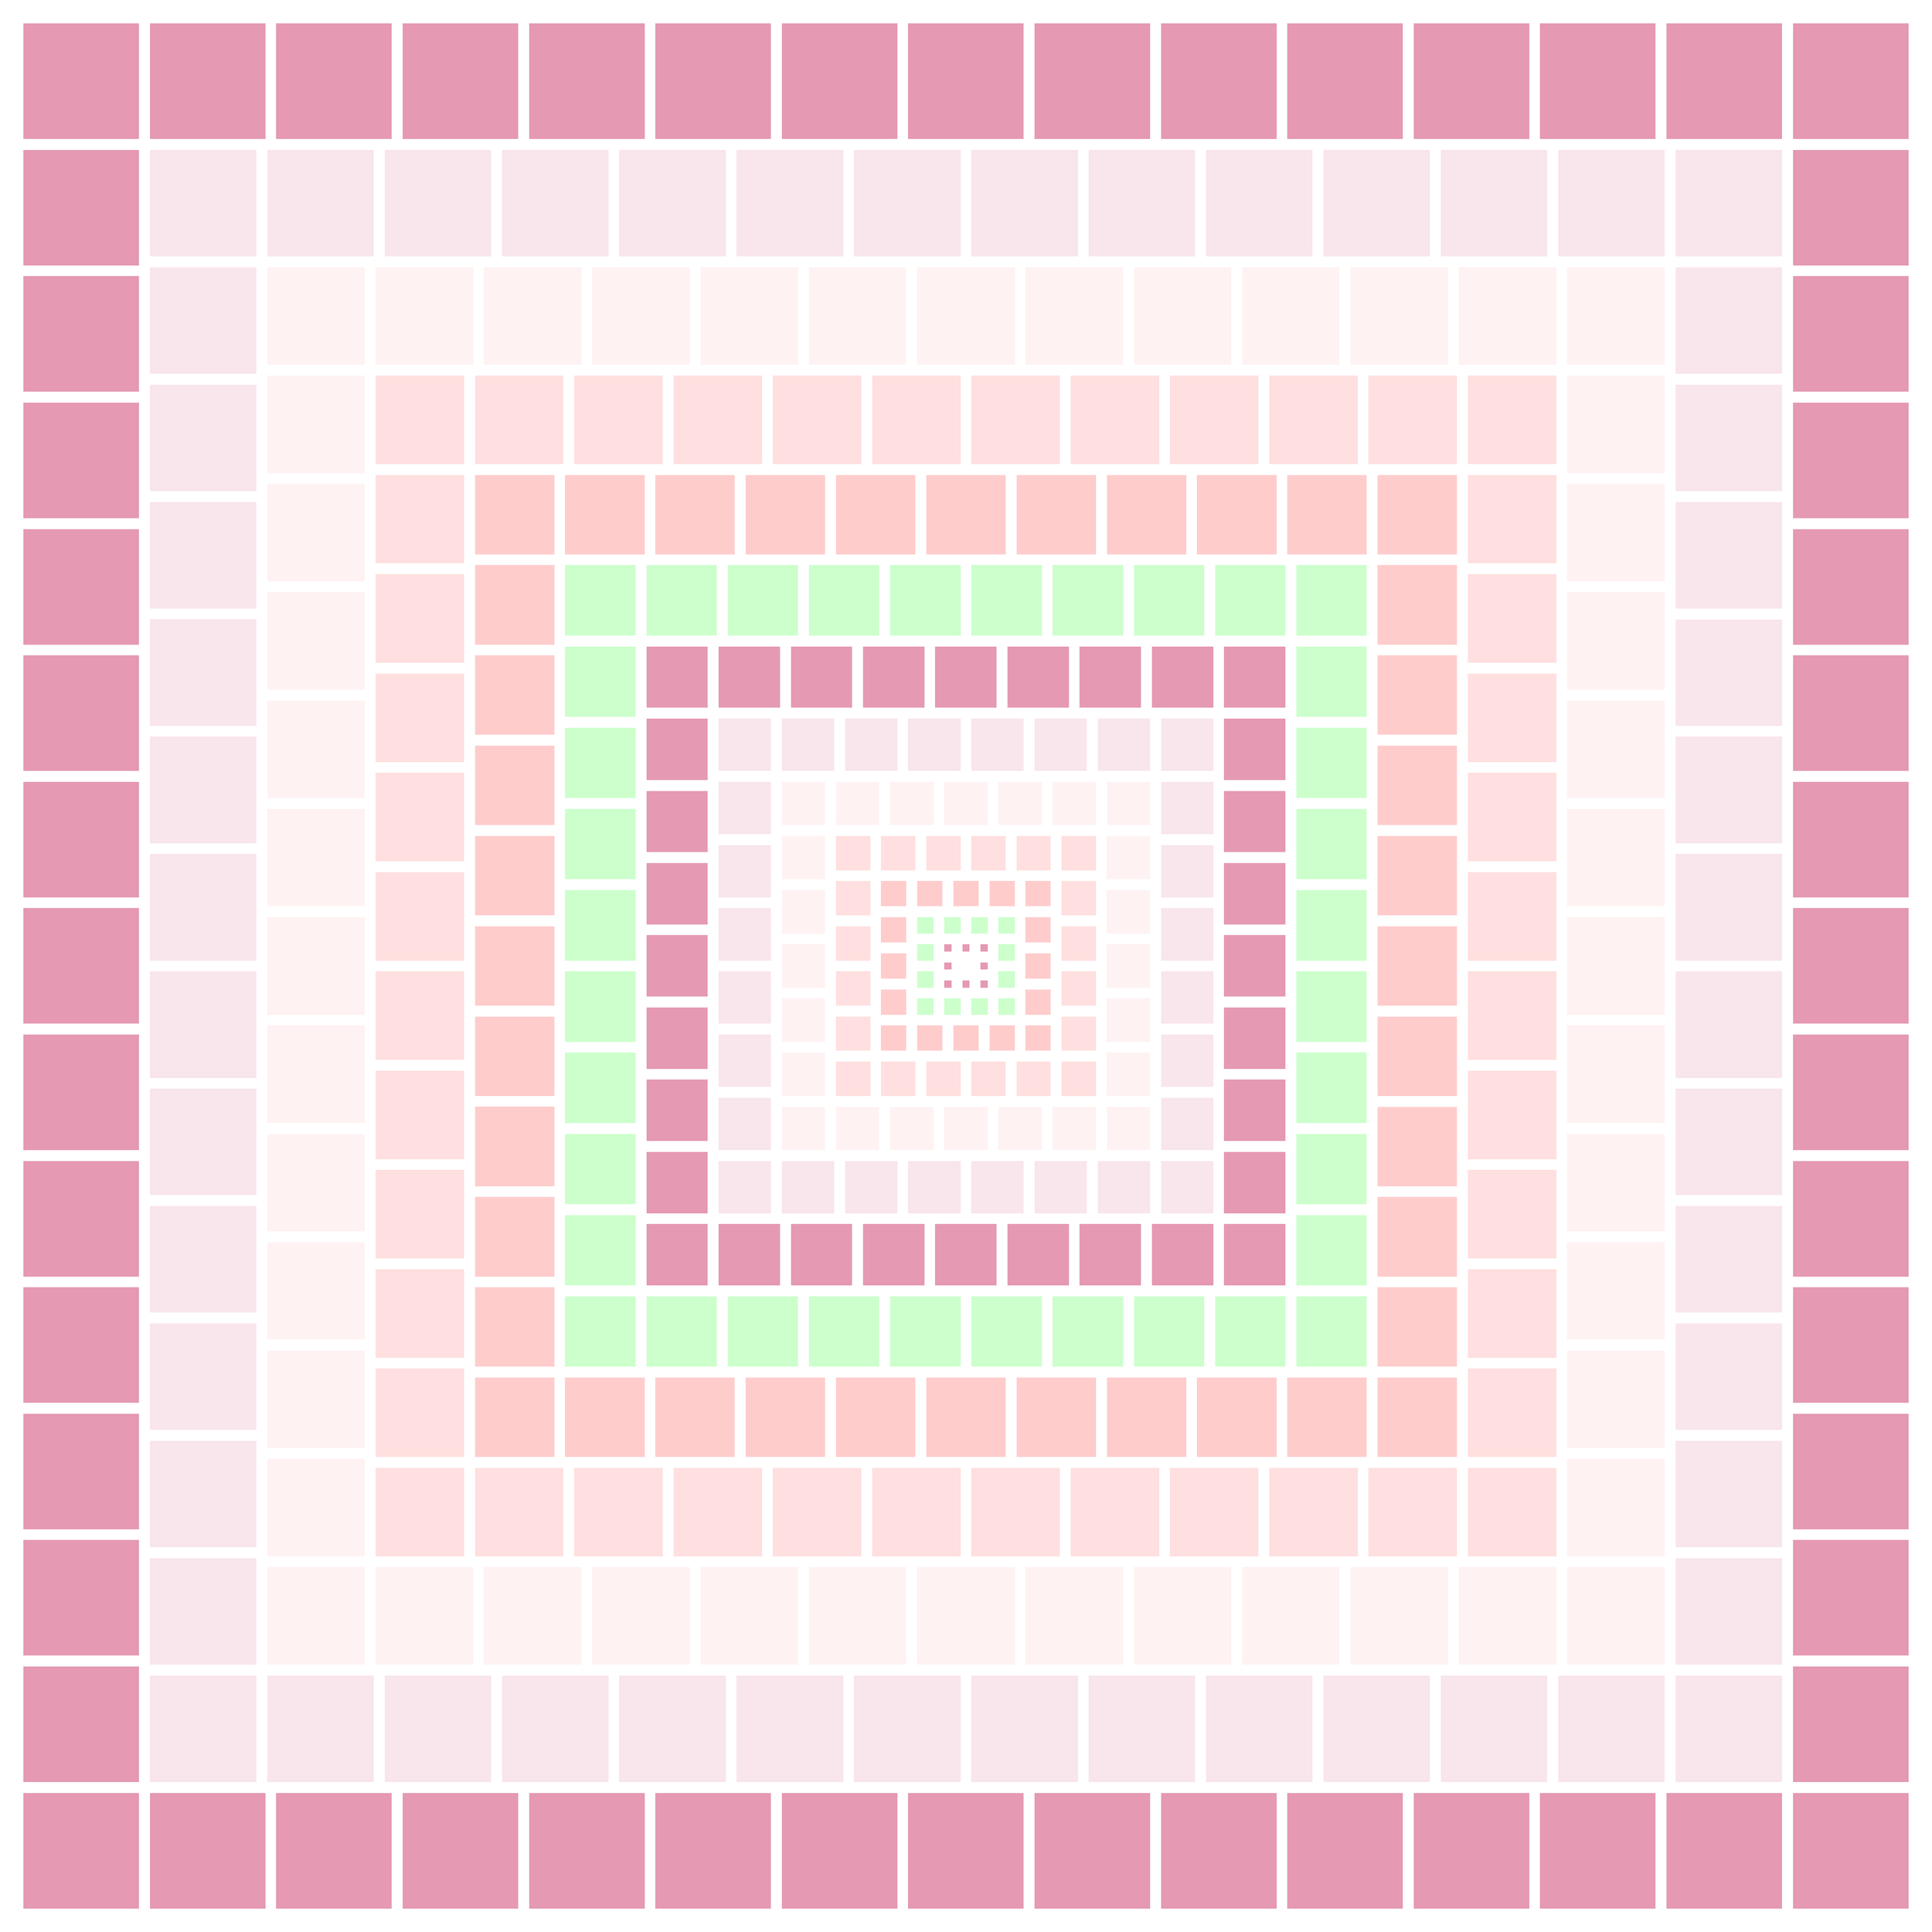
\begin{tikzpicture}[
	%tdplot_main_coords,
	scale=.5,
	line width=3mm,
	1/.style={fill=pink!50, draw=white},
	2/.style={fill=pink!20, draw=white},
	3/.style={fill=purple!10, draw=white},
	4/.style={fill=purple!40, draw=white},
	5/.style={fill=green!20, draw=white},
	6/.style={fill=red!20, draw=white},
	]

\def\lO{.5}


\path (0,0) coordinate(O);
\pgfmathsetmacro{\r}{sqrt(2*\lO*\lO)}
\foreach \a in {45,135,225,315}{
	\path (O)++(\a:\r)coordinate(\a);
}
\draw[2] (45)--(135)--(225)--(315)--cycle;
\draw[2] (O)++(-\lO,0)--++(\lO+\lO,0);
\draw[2] (O)++(0,-\lO)--++(0,\lO+\lO);

\def\N{15}

\foreach \n in {3,...,\N}{
	\pgfmathsetmacro{\l}{\lO*(\n-1)}
	\pgfmathsetmacro{\r}{sqrt(2*\l*\l)}
	\pgfmathtruncatemacro{\nn}{mod(\n, 6)+1}

	\path (225)++(225:\r) coordinate(X);
	\foreach \i in {1,...,\n}{
		\path[\nn] (X)--++(\l,0)coordinate(X)--++(0,\l)--++(-\l,0)--cycle;
	}
	\path (225)coordinate(X);
	\pgfmathtruncatemacro{\nx}{\n-2}
	\foreach \i in {1,...,\nx}{
		\path[\nn] (X)--++(0,\l)coordinate(X)--++(-\l,0)--++(0,-\l)--cycle;
	}
	\path (135)++(135:\r) coordinate(X);
	\foreach \i in {1,...,\n}{
		\path[\nn] (X)--++(\l,0)coordinate(X)--++(0,-\l)--++(-\l,0)--cycle;
	}
	\path (45)coordinate(X);
	\foreach \i in {1,...,\nx}{
		\path[\nn] (X)--++(0,-\l)coordinate(X)--++(\l,0)--++(0,\l)--cycle;
	}	

	\foreach \a in {45,135,225,315}{
		\path (\a)++(\a:\r)coordinate(\a);
	}
}



\end{tikzpicture}
\end{document}